% !TEX root = ../Survey.tex
	We discuss labeling schemes for \ancestry.
	First, we describe  a simple $2 \log n$ labeling scheme for the function, followed by literature review in Section~\ref{sec:anc-lit}.
	We then present a recent labeling scheme  of size $\log n + 2\log \log n$ in Section~\ref{subsetion:mat-optimal}.
	The bound is matched  asymptotically by a  lower bound, presented in Section~\ref{sub-anc-lower}.
	Finally, in Section~\ref{sub-anc-dynamic}, we  discuss dynamic \ancestry labeling schemes and present in detail a lower bound for a natural dynamic model.

		\paragraph{Na\"ive algorithm}\label{section:NaiveAncestry}
		The following $2 \log n $ \ancestry labeling scheme was introduced by \citeN{Kannan92}.
		Similarly to the one in Section~\ref{sec:example}, it is composed of  two numbers in the set $\{1 \dots n\}$.
		Using a $\dfs$ traversal (Section~\ref{sec:efficient-encoding}), the encoder assigns   node $v \in T$, with  $ \la(v) =  (\dfs(v),\dfs(w))$ where $w$ is the descendant of $u$ with largest $\dfs$ number  (if $v$ is a leaf we set $w=v$).
		 
		Encoding each label is done in a single $\dfs$ traversal.
		The resulting label $\la(v)=(\dfs(v),\dfs(w))$  represents an interval $I(v)$, where  $I(r) =  \{1 \dots n\}$.
		Given the labels $\la(u)$ and $\la(v)$ the decoder  returns true if  $I(v) \subseteq I(u)$.
		 See Figure~\ref{fig:simple-ancestry} for a demonstration of the labeling scheme.
			  
			  
\begin{figure}[!ht]
\centering
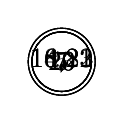
\begin{tikzpicture}[scale=0.7,inner sep=0pt, minimum size=5ex, sibling distance=0.4em]
\tikzstyle{every node}=[draw,circle]
\Tree  [ 
.{1,23} 
	\edge; [.{2,11} [.{3,10} \edge[]; [.{4,5} \node{5}; ]
							       [.\node{6,8}; \node{7}; \edge; {8} ]
                       					       \edge; [.{9,10} \node{10}; ]
					    ] 
					    \edge; {11} ]
	\edge;  [.{12,13} \node{13}; ]
	[.\node{14,23}; \edge; {15}
			[.\node{16,22}; \edge; {17}
					[.\node{18,21}; \edge; {19}
							\node{20};
							\edge; {21} ]
					\edge; {22} ]
			\edge; {23} ]
	]
\end{tikzpicture}
\caption{
A tree with $n=23$ nodes. Each node is assigned a label of size $2 \log n$ supporting \ancestry queries.} \label{fig:simple-ancestry}
\end{figure}
			
			
\subsection{Literature review}\label{sec:anc-lit}
	\ancestry  labeling schemes are typically classified into two categories; \emph{range-based} and \emph{prefix-based}.
	  \emph{Range-based} labels, such as the na\"ive labeling scheme, are decoded by  comparing the  ranges assigned to each node. An additional example of a range-based  labeling scheme is found in Section~\ref{subsetion:mat-optimal}.
	 \emph{Prefix-based} labels are decoded by comparing the prefix of both labels such that $u$ is an ancestor of $v$ if and only if $\la(u)$ is  a prefix of $\la(v)$.
	 An example of prefix-based labeling scheme is found in Section~\ref{sub-anc-dynamic}.
	  
	The $2\log n$ labeling  scheme presented above was improved gradually.
	 Abiteboul, Kaplan and Milo \shortcite{Kaplan01} achieved an upper bound of  $3/2 \log n +O(\log \log n)$ bits, which was improved  to $\log n + O(\sqrt{\log n})$~\cite{Alstrup06}.
	 Shortly after,  Alstrup and Bille \shortcite{Alstrup05} constructed a lower bound of $ \log n + \log \log n$ for any labeling scheme supporting the function.
	\citeN{Fraigniaud10} showed that $Trees(n, \delta)$ enjoy a labeling scheme of $ \log n+ O(\log \delta)$.
	The result was  generalised in a follow up paper~\cite{Korman10} for $Trees(n)$ in a labeling scheme of size $\log n+ 4 \log \log n $, which is asymptotically optimal. The bound was improved last by~\citeN{knudsen2014private} to $\log n + 2 \log \log n$.
	 Interestingly, the asymptotically optimal  labeling scheme  is based on  the first one presented eighteen years prior \cite{Kannan92}.
	
	In the case where \ancestry may be determined if the distance between the nodes is at most $d$, \citeN{Alstrup05} constructed a labeling scheme
	 of size $\log n + O( d \sqrt{ \log n})$, for which the new upper bound performs better for any $d$.
	 
	 Due to their great applicability in queries for XML documents, a staggering number of papers address this practical aspect~\cite{kaplan2002comparison,wu2004prime,o2004ordpaths,li2005qed,lu2005region,harder2007node,harder2007node,xu2009dde,cohen2010labeling,o2012scooter,ghaleb2013novel}.
	 Typically, those address the dynamic variant thereof.  For a short survey on  dynamic \ancestry labeling schemes, see~\cite{cohen2010labeling}.
	 
\subsection{Upper bound} \label{subsetion:mat-optimal}
In this section we prove the following.
  \begin{theorem}
  There exist a $\log n + 2\log \log n + O(1)$ \ancestry labeling scheme for $Trees(n)$.
  \end{theorem}
  
The  na\"ive labeling scheme presented above stores a two part label  $(x_v,y_v)$ for every node $v$ in a tree $T$ that represent the  interval $\{x_v \dots y_v\}$ of size $y_v-x_v+1$. Both  $x_v$ and $y_v$ may be any number in  $\{1 \dots n\}$ and therefore the label size is at most $2\log n$. The label  can also be stored in the form $(x_v,y_v-x_v+1)$ as demonstrated by the following pseudo code. 
The function computes a value $a$   for every node $v \in T$ specifying the largest $x_{v'}$ for any $v'$  in the subtree rooted in $v$. 
The function is initially called on  the root $r$  of $T$ and $\Id= 1$. 

\begin{algorithmic}[1] \Function{na\"ive}{node $v$, integer $\Id$}
        \State $a \gets \Id$	
	\ForAll{$l \in \children(v)$}   
	\State $a \gets  \Call{na\"ive}{l,a+1}$ 
	\EndFor
	\State $v.label \gets (\Id,(a-\Id))$ 
	\State \Return $a$  
\EndFunction
\end{algorithmic}


To reduce the label size further, we do not store $y_v-x_v+1$ explicitly. 
Instead, we use  an approximation  of that value that  requires only $O(\log \log n)$ bits. 
The value $x_v$ is now computed using an updated variant of the $\dfsi$ traversal (Section~\ref{sec:efficient-encoding}).
In particular, the order of the traversal remains the same.
While $x_v \geq \dfsi(v)$, it will  still hold that $x_v = O(n)$.

 As described in  Section~\ref{section:Misc-Tools}, we can store a $1+\frac{1}{2^k}$ approximation of any number in the range $\{1 \dots n\}$ using   $\log  \log n + k$ bits. The following labeling scheme uses $1+\frac{1}{2^k}$ approximation for carefully  chosen $k$.  For brevity, we now  denote $\frac{1}{2^k}$ by  $\epsilon$, and call $\app(x)$ the function that returns a $1+\epsilon$ approximation of an integer $x$.
Notice that  $ \log \log  x + \log\frac{1}{\epsilon}$ bits are required  to store the result of the function.

The label of a node $v$ in a rooted tree $T$ consists of the following two parts  $\la(v) = (\Id(v), \Ap(v))$.
For every node $v \in T$ the function \textsc{improved}  computes  two values, $a$ and $b$: in this $a$ stands for the largest number assigned and $b$ the largest number reserved  in the subtree rooted in $v$.
We initially call the  recursive  function using  the root of $T$ and $\Id = 1$. 

\begin{algorithmic}[1] \Function{improved}{node $v$, integer $\Id$}
        \State $(a,b) \gets (\Id,\Id)$	
	\ForAll{$l \in \children(v)$ in   increasing ordered size}   
	\State $(a,b) \gets  \Call{improved}{l,b+1}$ 
	\EndFor
	\State $v.label \gets (\Id,\app(a-\Id))$ 
	\State \Return $(a,\max{ \{b,\app(a-\Id)+\Id\}})$  \label{line:critical}
\EndFunction
\end{algorithmic}
   To prove that the encoder assigns labels of the requested size we first use  lemma~\ref{Lemma:newwriting}.
Recall  that $\ldepth(v)$ is the number of light nodes encountered on the path $r \leadsto v$, and that  the  $\ldepth(T)$ is the maximum light depth among the nodes in the tree $T$ (Section~\ref{tec:heavylight}). 
Recall also  that a node $v$ in a  tree $T$ roots the subtree $T(v)$ of size $\size(v)$.
\begin{lemma}\label{Lemma:newwriting}
Let $v$ be  a node in a tree $T$  of size $S = \size(v)$,   $x$ be an integer, and $l = \floor{\log S}$.
If $(a,b)=\textsc{improved}(v,x)$ then:
\begin{enumerate}
	\item $a \leq x + S(1+\epsilon)^l -1.$
	\item $b \leq x + S(1+\epsilon)^{l+1}-1.$
\end{enumerate}
\end{lemma}
\begin{proof}
		We prove the claims by induction over $l$, where the claims hold trivially for $l =1$.
		Assume that both claims hold for $l-1$  and we show that it holds for $l$.
		The children of $v$ are denoted $w_1 \dots w_k$ according to their size, where $w_k$ is the heavy node.
		The $a$ and $b$ values of  node $w_i$ are called $a_i$ and $b_i$ respectively.
		Since $w_1 \dots w_{k-1}$ are light nodes, $\size(w_1) \dots \size(w_{k-1}) < \frac{1}{2}S$, which implies that  $\floor{\log \size(w_i)} \leq l-1$.
		Thus, by the induction hypothesis  $b_1 \leq  x + \size(w_1)(1+\epsilon)^{l}-1$. 
		For both manners of  assigning $b_2$ (line~\ref{line:critical}) it now holds that,  
		$$b_2 \leq  b_1+1 + \size(w_2)(1+\epsilon)^{l}-1 \leq  X + (\size(w_1)+\size(w_2)) (1+\epsilon)^{l}-1.$$
		Applying the argument to all $b_i$ $3 \leq i \leq k-1$ we get:
		 $$b_{k-1} \leq   x +  \sum_{i=1}^{k-1}\size(w_i) (1+\epsilon)^{l}-1$$
	At this point  we can use the first hypothesis to get:
	$$a_{k} \leq  x +  \sum_{i=1}^{k-1}\size(w_i) (1+\epsilon)^{l} + \size(w_k)(1+\epsilon)^l$$
	Which is simply $S(1+\epsilon)^l-1$ As requested. The proof of the second argument is done similarly.
	\end{proof}
 
Since $l = \floor{\log S} \leq \log n$, by Lemma~\ref{Lemma:newwriting} the  total interval required is of size at most $\floor{n \cdot (1+ \epsilon)^{\log n}}$.
  It follows that the size of the first label part is at most $ \log n +  \log n \cdot \log(1+ \epsilon)+O(1)$ and the size of the second part is at most $\log \log  n + \log\frac{1}{\epsilon}+O(1)$. Choosing $\epsilon = 1/ \log n$, these are bounded by $\log n + O(1)$ and   $2 \log \log n+O(1)$, respectively.
  
 The encoding is done similarly  to the na\"ive decoder.
  Given labels $(\Id(v),\Ap(v))$ and $(\Id(u),\Ap(u))$ of nodes $v$ and $u$, respectively, the node  $v$ is an ancestor of $u$ if and only if $\Id(v) \leq \Id(u) \leq \Id(v)+(1+\epsilon)^{\Ap(v)}$. 
 In this labeling scheme the interval of a node's  decedent  may be of equal size to the one used by the node. Therefore, unlike the na\"ive labeling scheme, the intervals are not necessarily  fully contained. 
 	
\subsection{Lower bound}\label{sub-anc-lower}
The following  lower bound is an extension of the one by \citeN{Alstrup05} using the same technique, namely, boxes and groups (Section~\ref{section:boxes-and-groups}). 
\begin{theorem} \label{theo:ancestrytreeslower}
For any $n,\delta$ with $n\geq \delta+1\geq 3$, any \ancestry labeling scheme for $Trees(n,\delta)$
has a worst-case label size of at least $\ceil{\log n} + \floor{\log \floor{\log \delta}}-1$.\footnote{Observe that the assumption $n\geq \delta+1$ is natural, since any tree with $n$ nodes and depth $\delta$ satisfies $n\geq \delta+1$.}
\end{theorem}
\begin{proof}
Let $m=2^{\floor{\log (n-1)}}=2^{\ceil{\log n}-1}$ be $n-1$ rounded down to the nearest power of $2$, and set $k=\floor{\log \delta}$. Note that $k\leq \log m$. Construct for $i=1\dots k$ the tree $T_i$ as a root node to which $m/2^i$ paths of length $2^i$ have been attached. Thus, $T_i$ has $m+1\leq n$ nodes, whereof $m$ belong to disjoint paths. Further, $T_i$ has depth $2^i\leq 2^k\leq \delta$, and hence $T_i$ belongs to $Trees(n,\delta)$. For an illustration of such trees see Figure~\ref{fig:TheosDrawing}.

Each node in a tree must be uniquely labeled by an \ancestry labeling scheme. Further, if two nodes in $T_i$ lie on distinct paths, then their labels cannot be used on the same path in $T_j$ for any  $j\neq i$, because nodes on the same path have an \ancestry relation whereas nodes on different paths do not. We can therefore apply Lemma~\ref{lemma:boxgroups}, using the $m$ nodes of the paths of each tree as a ``box'' and each path as a ``group'', and it follows that we need at least $\frac{1}{2}m(k+1) = \frac{1}{2}m(\floor{\log \delta}+1)$ labels. If the worst-case label size is $L$  we can create $2^{L+1}-1$ distinct labels, and we must therefore have $\frac{1}{2}m(\floor{\log \delta}+1)\leq 2^{L+1}-1$ from which it follows that $L\geq \ceil{\log n} + \floor{\log \floor{\log \delta}}-1$.
\end{proof}
			
			\begin{figure}[!ht] 
				\centering
				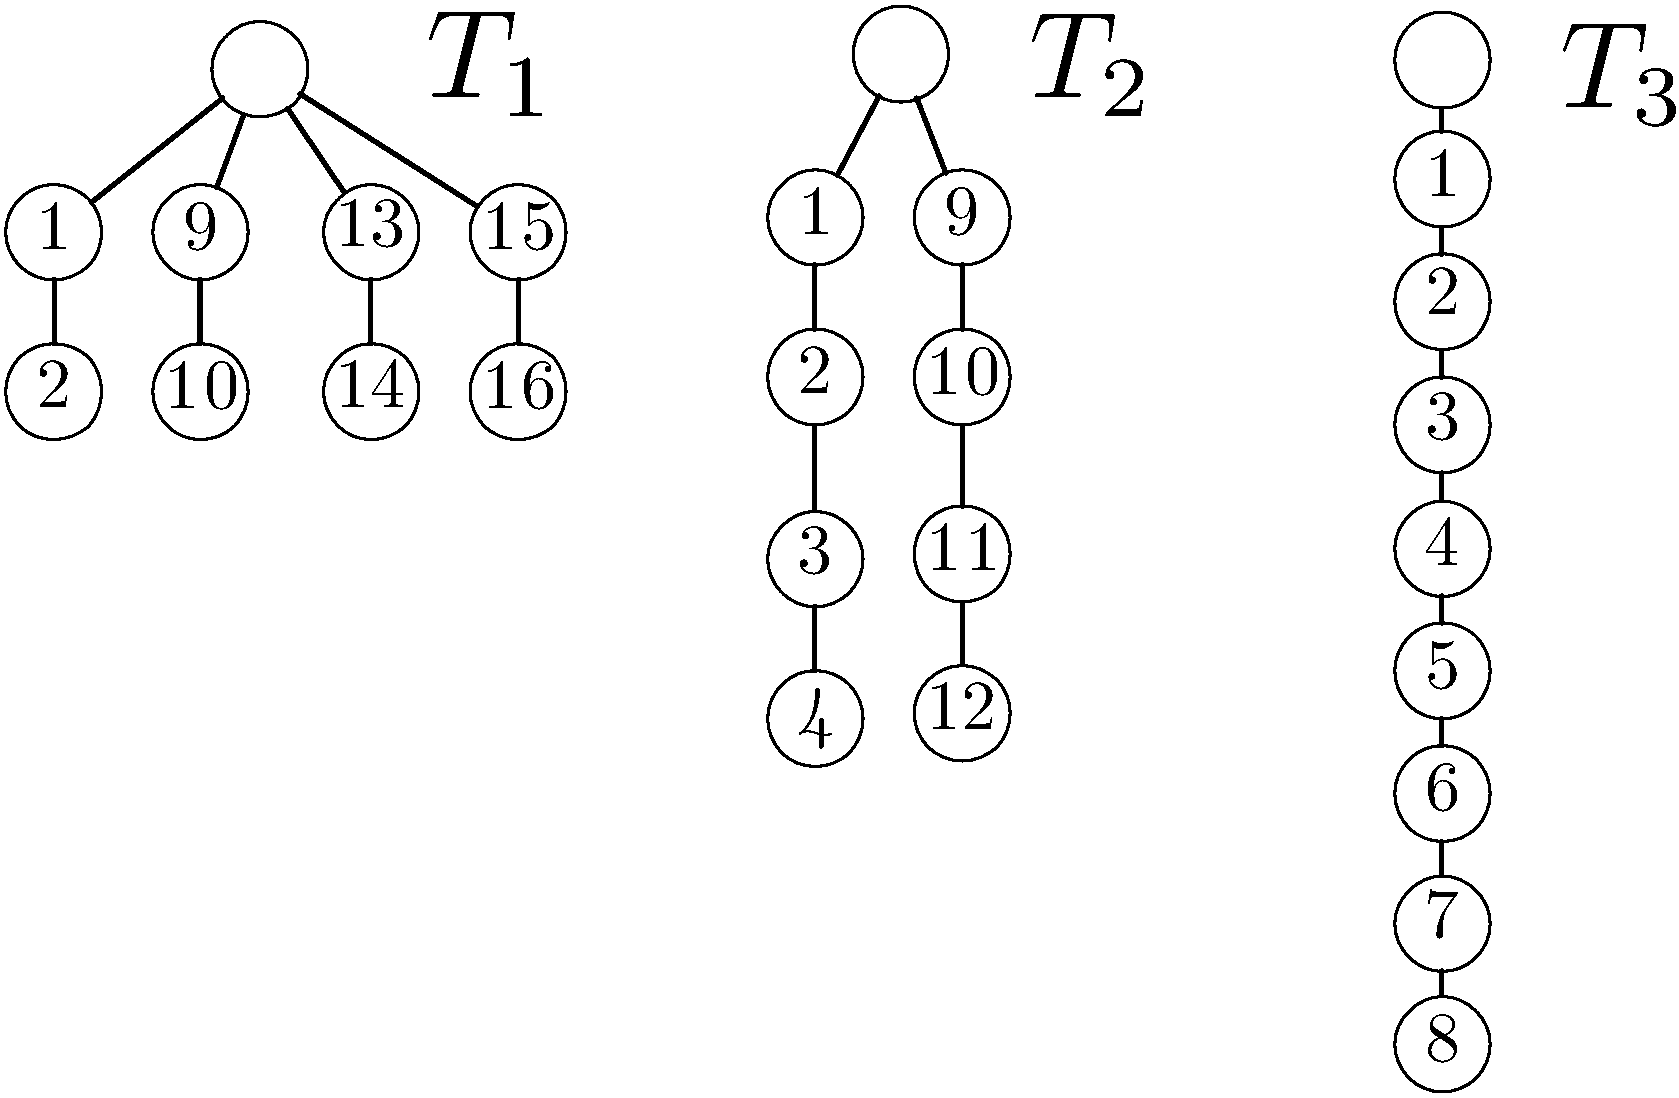
\includegraphics[width=60mm]{./Figures/Lowerbound-ancestry.pdf}
				\caption{Illustration of $T_1,T_2,T_3$ for $n=8$. }
				\label{fig:TheosDrawing}
			\end{figure}

%\subsection{Siblings and connectivity} \label{section:Sib}
%The lower bound presented above can be derived for the functions Siblings and connectivity.
%In contrast to ancestry, attaining a $\log n + \log \log n$ labeling scheme for both functions is easy.
%Moreover, if the labels are not necessarily unique, a straightforward $\log(n)$ labeling scheme exist for both.

\subsection{Dynamic \ancestry labeling schemes}	\label{sub-anc-dynamic}	
			All results described thus far in the survey present a worst-case analysis of static trees.
			We  describe the first dynamic result, in which rather than receiving a tree $T$, the decoder receives a sequence of $n$ operations constructing $T$.
			Operations considered in the literature are insertions  and deletions of leaves, or arbitrary nodes.
			For convenience  it is assumed that the sequence constructs a rooted tree, and its root exist from the beginning and  is never  deleted.
			
			The section discusses a  \emph{persistent} \ancestry labeling scheme, i.e a dynamic labeling scheme that does not change the label given to a node.
			The result is described in a model in which the operation allowed is an  insertion of  leaves.
			%For labeling schemes with permitted relabelling, as well as further implications of the result presented see Section~\ref{section:dynamic}.

			A trivial prefix-based labeling \ancestry labeling scheme for the model is  built directly from the suffix free  $code_0$ (Section~\ref{tec:suffix}).
			The root $r$ receives the label $1$. Suppose   node $v$ receives the label $\la(v)$. The $i$'th child of $v$ receives the label $\la(v) \circ 10^{i-1}$.
			Decoding $\la(u),\la(v)$ is done in the standard way, and the label size is at most $O(n)$.
			The next section proves that this trivial labeling scheme is asymptotically  optimal.
			
			\paragraph{Lower bound for persistent \ancestry labeling scheme}
			Cohen, Kaplan and Milo \shortcite{Cohen02} proved a lower bound of  $\Omega(n)$ on the label length for a sequence of $n+1$ insertions.
			They do so by presenting a family of insertion sequences of size $2^{n-1}$, such that each sequence has  at least one node with unique label.
			\begin{definition}\label{dfn:kaplans-trees}
			We define the family of insertion sequences $\mathcal{F}(n)$ recursively as follows.
				$\mathcal{F}(1)$ consists of a single sequence which inserts a root $r$ and a child of $r$, $w$.
				$\mathcal{F}(n)$ \textit{extends} each sequence $s$  in  $\mathcal{F}(n-1)$ rooted in $r$ to two sequences $s_1$ and $s_2$.
				Both insertion sequences replace the insertion of the root $r$ by the sequence $r'$ and $w'$,  a child of $r'$.
				$s_1$ is defined by connecting nodes previously adjacent to $r$  to be adjacent to  $w'$.
				In the same manner, $r'$ ``replaces'' $r$ in  $s_2$. 
				For illustration, see Figure~\ref{fig:KaplansTrees}.
			\end{definition}
			For convenience, we denote the last node in a sequence $s$, as $last(s)$, and the set of all sequences $s_2$, respectively~$s_1$ in $\mathcal{F}(n)$ created from $s \in \mathcal{F}(n-1)$ as  $s_2$ type sequence respectively~$s_1$ type sequence.	
			
			Since  $\vert \mathcal{F}(1) \vert = 1$, and  $\vert \mathcal{F}(i) \vert = 2 \cdot \vert \mathcal{F}(i-1) \vert $ it follows that the number of insertion sequences is $\vert \mathcal{F}(n) \vert = 2^{n-1}$.
			Each insertion sequence in $\mathcal{F}(n)$ has one more node than the sequence it was built upon from $\mathcal{F}(n-1)$. 
			Since the size of the sequence in $\mathcal{F}(1)$ is $2$, it follows that the size of each insertion sequence in $\mathcal{F}(n)$ is $n+1$.
			
			\begin{figure}[!ht] 
				\centering
				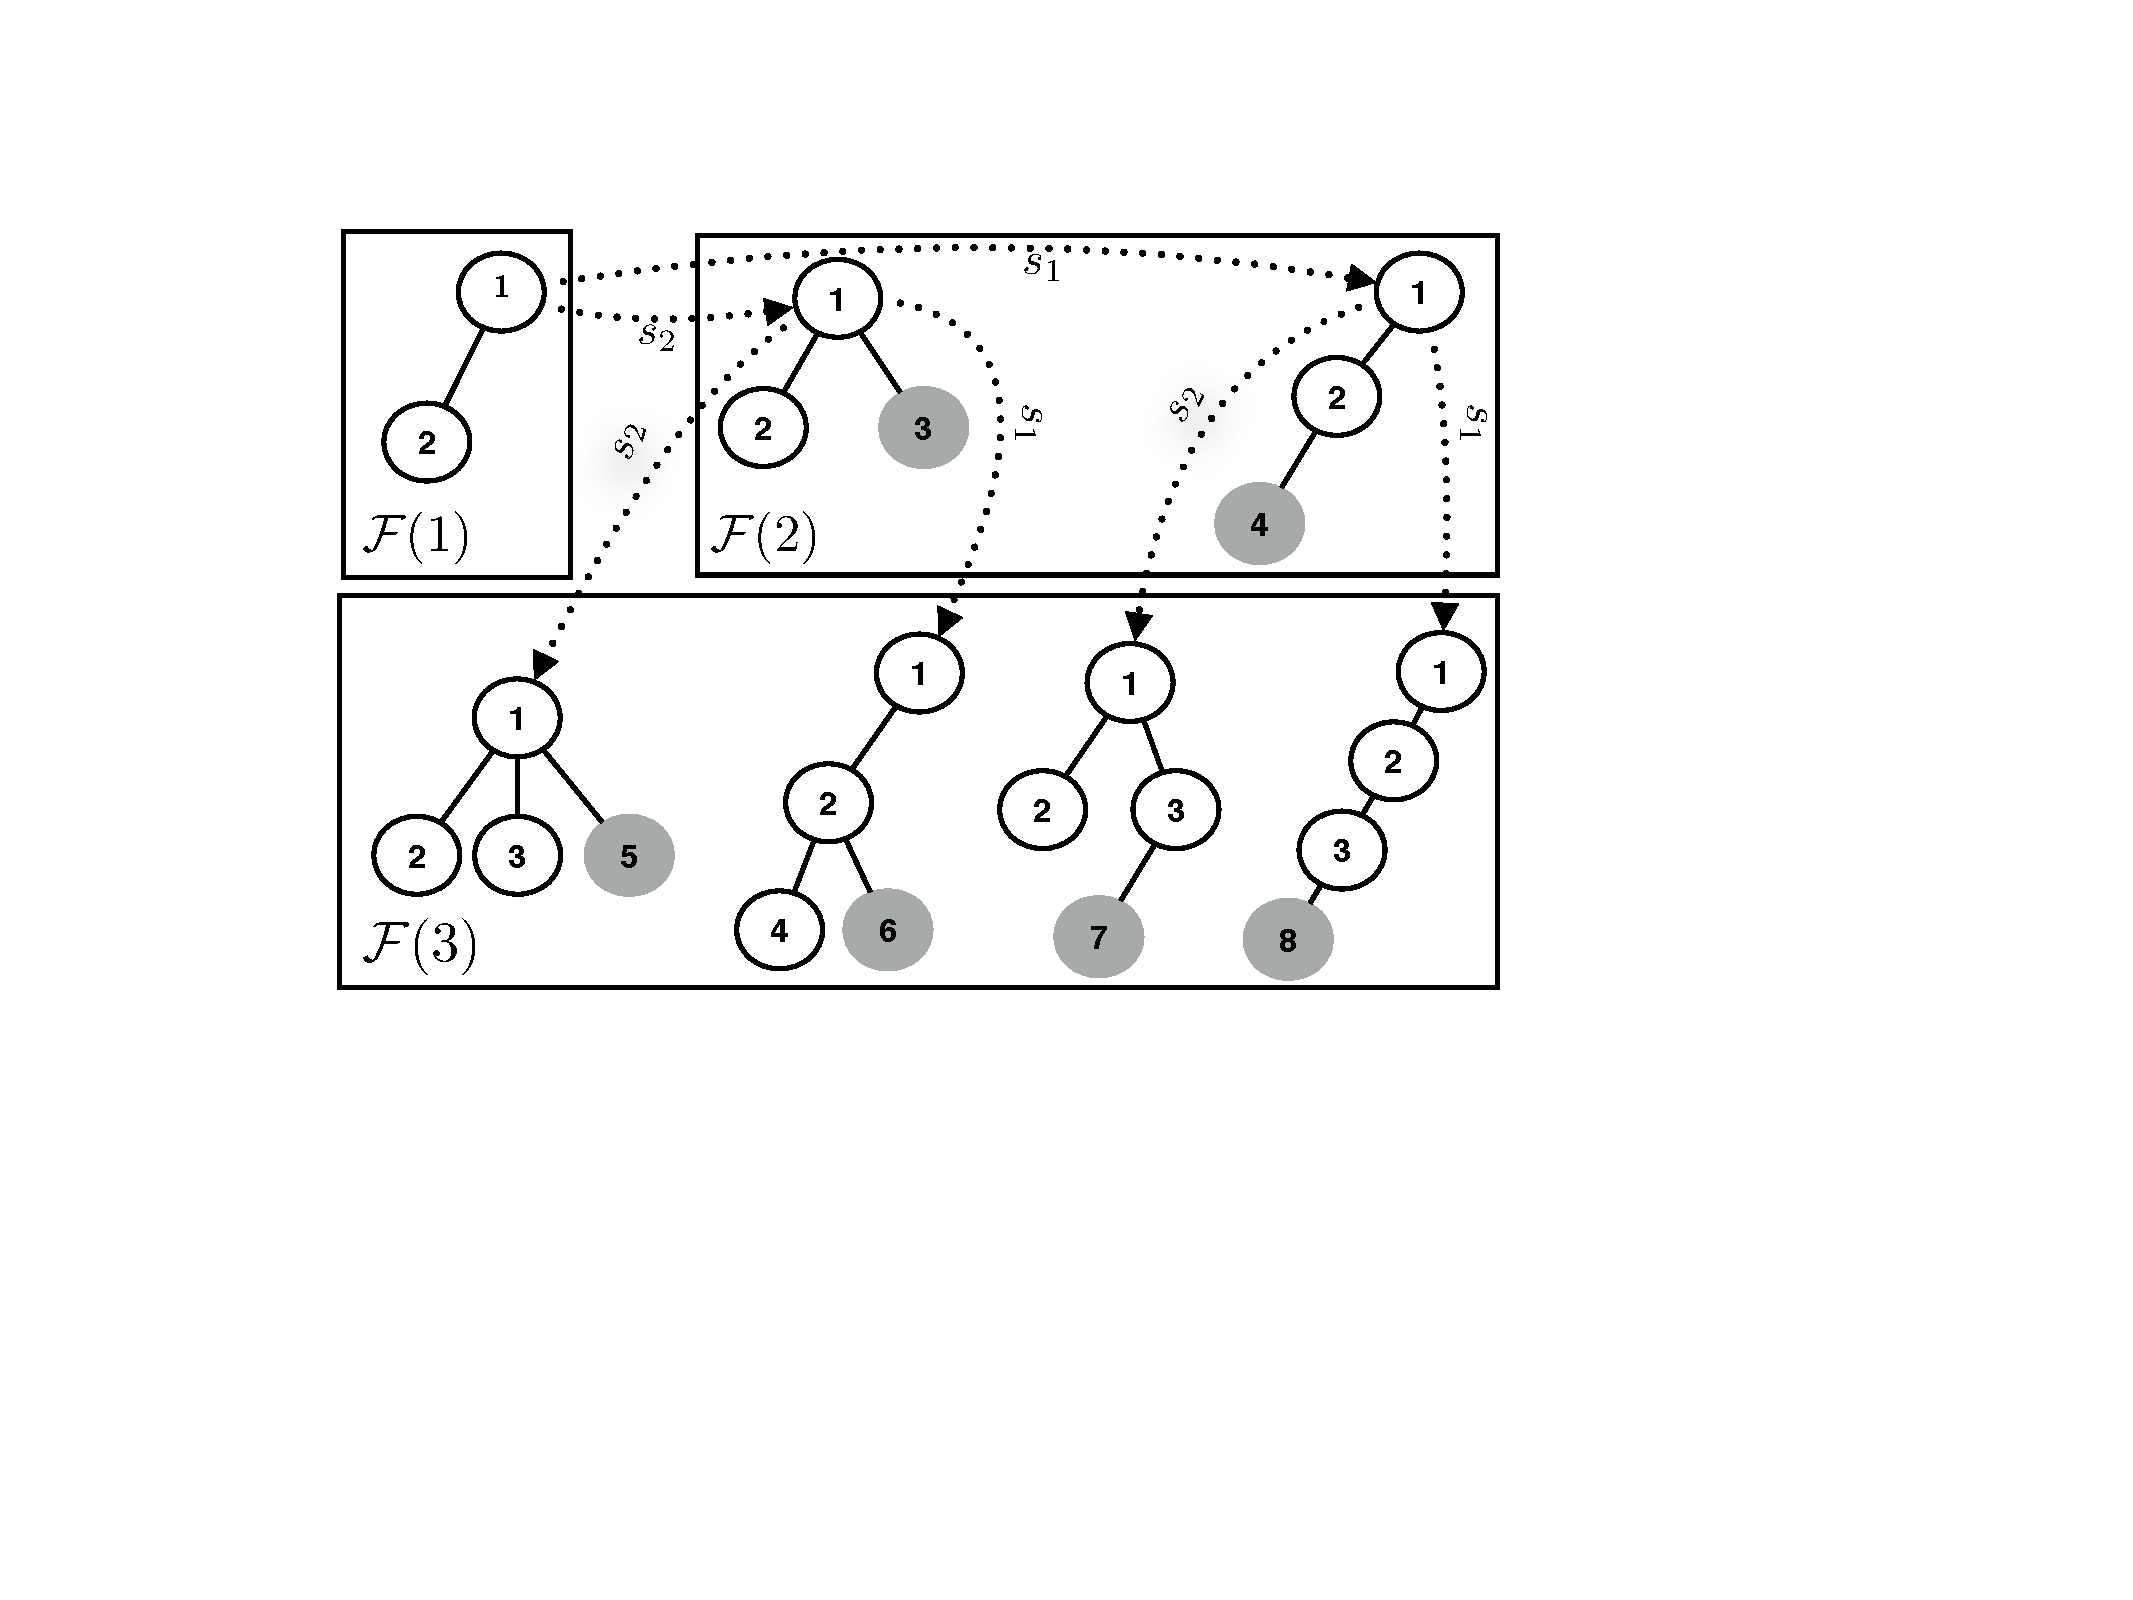
\includegraphics[width=70mm]{./Figures/Kaplans.pdf}
				\caption{ An illustration of  the trees resulting by the sequences $\mathcal{F}(1)$,  $\mathcal{F}(2)$ and  $\mathcal{F}(3)$ from Definition~\ref{dfn:kaplans-trees}. The grey nodes are the ones introduced by Lemma~\ref{lemma:persistent}.
				The arrows denote the extension of a sequence, and marked $s_1$ or $s_2$ according to the type.}
				\label{fig:KaplansTrees}
			\end{figure}
			
			We proceed to present the lower bound.
			\begin{lemma}\label{lemma:persistent}\cite{Kaplan01}
				Any  persistent  \ancestry labeling scheme with a deterministic encoder must give a unique label to the last insertion in  each of the  insertion sequences in $\mathcal{F}(n)$. 
			\end{lemma}

			\begin{proof}
				The claim is proved by induction.
				Suppose the claim is true for $\mathcal{F}(n-1)$, and pick two  insertion sequences $s, s' \in \mathcal{F}(n-1)$.
				 Denote the  sequences  extending  $s$ and $s'$ using  the first extension  type $s_1$ and $s'_1$ respectively.
				From the induction hypothesis it follows directly that $\la(last(s_1)) \neq \la(last(s_1'))$. %An illustration thereof is available in Fig.~\ref{fig:KaplansTrees}.
				
				Denote now both  derived sequences of $s$ in $\mathcal{F}(n)$ as  $s_1$ and $s_2$.
				Since the encoder is deterministic, and the first two elements of the insertions are identical,  $r'$ and $w'$ receives the same label in both.
				The node $last(s_1)$ is not a decedent of $w$ but $last(s_2)$ is.
				 Since the decoder needs to determine an \ancestry relation, $d(\la(w),\la(last(s_1))) = false$ and $d(\la(w),\la(last(s_2))) = true$.
				  Therefore, it is required that $\la(last(s_1)) \neq \la(last(s_2))$. 
			\end{proof}
				
				From Lemma~\ref{lemma:persistent}, and since there are $2^{n-1}$ insertion sequences of size $n$, it follows that $2^{n-1}$ distinct labels are needed for the last node in each sequence in $\mathcal{F}(n)$.
			\begin{corollary} \label{cor:persistent}
				Every persistent \ancestry labeling scheme  $\tuple{e,d}$ is of size $\Omega(n)$.
			\end{corollary}
			Using a similar argument, \citeN{Cohen02}  prove that the bound  holds for  a sequence corresponding to a tree from $Trees(n,\Delta)$, when $\Delta \geq 2$.
			Moreover, the bound is shown to hold even when the encoder is allowed to use randomisation.
			

		To overcome this inherent difficulty, the authors introduce the notion of \emph{sibling} and \emph{direct clues}.
			Loosely speaking, sibling, respectively, direct clues provide every node $v$ in the sequence a guarantee on the  range of possible number of $v$'s siblings, respectively~size of $v$.
		Using this method, they show tight bounds on the label sizes for such labeling schemes with  $\Theta(\log n)$ bits using sibling clues  and  $\Theta( \log^2 n)$ bits using direct clues. \citeN{dahlgaard2014dynamic} showed that this bound applies for the functions \NCA, \distance, and \routing as well. In contrast, they showed that $2 \log n$ are sufficient and necessary in this model for the functions \adjacency, \siblings and \connectivity.	
			

